% Options for packages loaded elsewhere
\PassOptionsToPackage{unicode}{hyperref}
\PassOptionsToPackage{hyphens}{url}
%
\documentclass[
  11pt,
]{article}
\usepackage{lmodern}
\usepackage{amsmath}
\usepackage{ifxetex,ifluatex}
\ifnum 0\ifxetex 1\fi\ifluatex 1\fi=0 % if pdftex
  \usepackage[T1]{fontenc}
  \usepackage[utf8]{inputenc}
  \usepackage{textcomp} % provide euro and other symbols
  \usepackage{amssymb}
\else % if luatex or xetex
  \usepackage{unicode-math}
  \defaultfontfeatures{Scale=MatchLowercase}
  \defaultfontfeatures[\rmfamily]{Ligatures=TeX,Scale=1}
\fi
% Use upquote if available, for straight quotes in verbatim environments
\IfFileExists{upquote.sty}{\usepackage{upquote}}{}
\IfFileExists{microtype.sty}{% use microtype if available
  \usepackage[]{microtype}
  \UseMicrotypeSet[protrusion]{basicmath} % disable protrusion for tt fonts
}{}
\makeatletter
\@ifundefined{KOMAClassName}{% if non-KOMA class
  \IfFileExists{parskip.sty}{%
    \usepackage{parskip}
  }{% else
    \setlength{\parindent}{0pt}
    \setlength{\parskip}{6pt plus 2pt minus 1pt}}
}{% if KOMA class
  \KOMAoptions{parskip=half}}
\makeatother
\usepackage{xcolor}
\IfFileExists{xurl.sty}{\usepackage{xurl}}{} % add URL line breaks if available
\IfFileExists{bookmark.sty}{\usepackage{bookmark}}{\usepackage{hyperref}}
\hypersetup{
  pdftitle={Summarizing The Weather},
  hidelinks,
  pdfcreator={LaTeX via pandoc}}
\urlstyle{same} % disable monospaced font for URLs
\usepackage[margin=1in]{geometry}
\usepackage{color}
\usepackage{fancyvrb}
\newcommand{\VerbBar}{|}
\newcommand{\VERB}{\Verb[commandchars=\\\{\}]}
\DefineVerbatimEnvironment{Highlighting}{Verbatim}{commandchars=\\\{\}}
% Add ',fontsize=\small' for more characters per line
\usepackage{framed}
\definecolor{shadecolor}{RGB}{248,248,248}
\newenvironment{Shaded}{\begin{snugshade}}{\end{snugshade}}
\newcommand{\AlertTok}[1]{\textcolor[rgb]{0.94,0.16,0.16}{#1}}
\newcommand{\AnnotationTok}[1]{\textcolor[rgb]{0.56,0.35,0.01}{\textbf{\textit{#1}}}}
\newcommand{\AttributeTok}[1]{\textcolor[rgb]{0.77,0.63,0.00}{#1}}
\newcommand{\BaseNTok}[1]{\textcolor[rgb]{0.00,0.00,0.81}{#1}}
\newcommand{\BuiltInTok}[1]{#1}
\newcommand{\CharTok}[1]{\textcolor[rgb]{0.31,0.60,0.02}{#1}}
\newcommand{\CommentTok}[1]{\textcolor[rgb]{0.56,0.35,0.01}{\textit{#1}}}
\newcommand{\CommentVarTok}[1]{\textcolor[rgb]{0.56,0.35,0.01}{\textbf{\textit{#1}}}}
\newcommand{\ConstantTok}[1]{\textcolor[rgb]{0.00,0.00,0.00}{#1}}
\newcommand{\ControlFlowTok}[1]{\textcolor[rgb]{0.13,0.29,0.53}{\textbf{#1}}}
\newcommand{\DataTypeTok}[1]{\textcolor[rgb]{0.13,0.29,0.53}{#1}}
\newcommand{\DecValTok}[1]{\textcolor[rgb]{0.00,0.00,0.81}{#1}}
\newcommand{\DocumentationTok}[1]{\textcolor[rgb]{0.56,0.35,0.01}{\textbf{\textit{#1}}}}
\newcommand{\ErrorTok}[1]{\textcolor[rgb]{0.64,0.00,0.00}{\textbf{#1}}}
\newcommand{\ExtensionTok}[1]{#1}
\newcommand{\FloatTok}[1]{\textcolor[rgb]{0.00,0.00,0.81}{#1}}
\newcommand{\FunctionTok}[1]{\textcolor[rgb]{0.00,0.00,0.00}{#1}}
\newcommand{\ImportTok}[1]{#1}
\newcommand{\InformationTok}[1]{\textcolor[rgb]{0.56,0.35,0.01}{\textbf{\textit{#1}}}}
\newcommand{\KeywordTok}[1]{\textcolor[rgb]{0.13,0.29,0.53}{\textbf{#1}}}
\newcommand{\NormalTok}[1]{#1}
\newcommand{\OperatorTok}[1]{\textcolor[rgb]{0.81,0.36,0.00}{\textbf{#1}}}
\newcommand{\OtherTok}[1]{\textcolor[rgb]{0.56,0.35,0.01}{#1}}
\newcommand{\PreprocessorTok}[1]{\textcolor[rgb]{0.56,0.35,0.01}{\textit{#1}}}
\newcommand{\RegionMarkerTok}[1]{#1}
\newcommand{\SpecialCharTok}[1]{\textcolor[rgb]{0.00,0.00,0.00}{#1}}
\newcommand{\SpecialStringTok}[1]{\textcolor[rgb]{0.31,0.60,0.02}{#1}}
\newcommand{\StringTok}[1]{\textcolor[rgb]{0.31,0.60,0.02}{#1}}
\newcommand{\VariableTok}[1]{\textcolor[rgb]{0.00,0.00,0.00}{#1}}
\newcommand{\VerbatimStringTok}[1]{\textcolor[rgb]{0.31,0.60,0.02}{#1}}
\newcommand{\WarningTok}[1]{\textcolor[rgb]{0.56,0.35,0.01}{\textbf{\textit{#1}}}}
\usepackage{longtable,booktabs}
\usepackage{calc} % for calculating minipage widths
% Correct order of tables after \paragraph or \subparagraph
\usepackage{etoolbox}
\makeatletter
\patchcmd\longtable{\par}{\if@noskipsec\mbox{}\fi\par}{}{}
\makeatother
% Allow footnotes in longtable head/foot
\IfFileExists{footnotehyper.sty}{\usepackage{footnotehyper}}{\usepackage{footnote}}
\makesavenoteenv{longtable}
\usepackage{graphicx}
\makeatletter
\def\maxwidth{\ifdim\Gin@nat@width>\linewidth\linewidth\else\Gin@nat@width\fi}
\def\maxheight{\ifdim\Gin@nat@height>\textheight\textheight\else\Gin@nat@height\fi}
\makeatother
% Scale images if necessary, so that they will not overflow the page
% margins by default, and it is still possible to overwrite the defaults
% using explicit options in \includegraphics[width, height, ...]{}
\setkeys{Gin}{width=\maxwidth,height=\maxheight,keepaspectratio}
% Set default figure placement to htbp
\makeatletter
\def\fps@figure{htbp}
\makeatother
\setlength{\emergencystretch}{3em} % prevent overfull lines
\providecommand{\tightlist}{%
  \setlength{\itemsep}{0pt}\setlength{\parskip}{0pt}}
\setcounter{secnumdepth}{5}
\ifluatex
  \usepackage{selnolig}  % disable illegal ligatures
\fi

\title{Summarizing The Weather}
\author{}
\date{\vspace{-2.5em}4/23/2021}

\begin{document}
\maketitle

{
\setcounter{tocdepth}{2}
\tableofcontents
}
\hypertarget{setup-and-libraries}{%
\section{Setup and Libraries}\label{setup-and-libraries}}

\begin{Shaded}
\begin{Highlighting}[]
\FunctionTok{library}\NormalTok{(magrittr)}
\FunctionTok{library}\NormalTok{(lubridate)}
\end{Highlighting}
\end{Shaded}

\begin{verbatim}
## 
## Attaching package: 'lubridate'
\end{verbatim}

\begin{verbatim}
## The following objects are masked from 'package:base':
## 
##     date, intersect, setdiff, union
\end{verbatim}

\hypertarget{introduction}{%
\section{Introduction}\label{introduction}}

This Code Clinic problem is about calculating statistics from a data
set. It's easy stuff, but presents a good example of how different
languages accomplish common tasks.

\hypertarget{import-the-source-data}{%
\section{Import the source data}\label{import-the-source-data}}

The data set is weather data captured from Lake Pend O'Reille in
Northern Idaho. We have almost 20 megabytes of data from the years 2012
thorugh 2015. That data is available in the folder with other exercise
files. Each observation in the data includes several variables and the
data is straightforward.

\begin{Shaded}
\begin{Highlighting}[]
\NormalTok{mytempfile }\OtherTok{\textless{}{-}} \FunctionTok{tempfile}\NormalTok{()}

\NormalTok{readOneFile }\OtherTok{\textless{}{-}} \ControlFlowTok{function}\NormalTok{(dataPath) \{}
  \FunctionTok{read.table}\NormalTok{(dataPath,}
             \AttributeTok{header =} \ConstantTok{TRUE}\NormalTok{,}
             \AttributeTok{stringsAsFactors =} \ConstantTok{FALSE}\NormalTok{)}
\NormalTok{\}}

\NormalTok{myProgressBar }\OtherTok{\textless{}{-}} \FunctionTok{txtProgressBar}\NormalTok{(}\AttributeTok{min =} \DecValTok{2012}\NormalTok{, }\AttributeTok{max =} \DecValTok{2015}\NormalTok{, }\AttributeTok{style =} \DecValTok{3}\NormalTok{)}

\ControlFlowTok{for}\NormalTok{ (dataYear }\ControlFlowTok{in} \DecValTok{2012}\SpecialCharTok{:}\DecValTok{2015}\NormalTok{) \{}
  
\NormalTok{  dataPath }\OtherTok{\textless{}{-}}
    \FunctionTok{paste0}\NormalTok{(}
      \StringTok{"https://raw.githubusercontent.com/lyndadotcom/LPO\_weatherdata/master/Environmental\_Data\_Deep\_Moor\_"}\NormalTok{,}
\NormalTok{      dataYear,}
      \StringTok{".txt"}
\NormalTok{    )}
  
  \ControlFlowTok{if}\NormalTok{ (}\FunctionTok{exists}\NormalTok{(}\StringTok{"LPO\_weather\_data"}\NormalTok{)) \{}
\NormalTok{    mytempfile }\OtherTok{\textless{}{-}} \FunctionTok{readOneFile}\NormalTok{(dataPath)}
\NormalTok{    LPO\_weather\_data }\OtherTok{\textless{}{-}} \FunctionTok{rbind}\NormalTok{(LPO\_weather\_data, mytempfile)}
\NormalTok{  \} }\ControlFlowTok{else}\NormalTok{ \{}
\NormalTok{    LPO\_weather\_data }\OtherTok{\textless{}{-}} \FunctionTok{readOneFile}\NormalTok{(dataPath)}
\NormalTok{  \}}
  \FunctionTok{setTxtProgressBar}\NormalTok{(myProgressBar, }\AttributeTok{value =}\NormalTok{ dataYear)}
  
\NormalTok{\}}
\end{Highlighting}
\end{Shaded}

\begin{verbatim}
##   |                                                                              |                                                                      |   0%  |                                                                              |=======================                                               |  33%  |                                                                              |===============================================                       |  67%  |                                                                              |======================================================================| 100%
\end{verbatim}

\begin{Shaded}
\begin{Highlighting}[]
\CommentTok{\# confirm the results of the import}
\FunctionTok{head}\NormalTok{(LPO\_weather\_data, }\AttributeTok{n =} \DecValTok{3}\NormalTok{)}
\end{Highlighting}
\end{Shaded}

\begin{longtable}[]{@{}llrrrrrrr@{}}
\toprule
\begin{minipage}[b]{(\columnwidth - 8\tabcolsep) * \real{0.11}}\raggedright
date\strut
\end{minipage} &
\begin{minipage}[b]{(\columnwidth - 8\tabcolsep) * \real{0.09}}\raggedright
time\strut
\end{minipage} &
\begin{minipage}[b]{(\columnwidth - 8\tabcolsep) * \real{0.09}}\raggedleft
Air\_Temp\strut
\end{minipage} &
\begin{minipage}[b]{(\columnwidth - 8\tabcolsep) * \real{0.16}}\raggedleft
Barometric\_Press\strut
\end{minipage} &
\begin{minipage}[b]{(\columnwidth - 8\tabcolsep) * \real{0.10}}\raggedleft
Dew\_Point\strut
\end{minipage} &
\begin{minipage}[b]{(\columnwidth - 8\tabcolsep) * \real{0.17}}\raggedleft
Relative\_Humidity\strut
\end{minipage} &
\begin{minipage}[b]{(\columnwidth - 8\tabcolsep) * \real{0.09}}\raggedleft
Wind\_Dir\strut
\end{minipage} &
\begin{minipage}[b]{(\columnwidth - 8\tabcolsep) * \real{0.10}}\raggedleft
Wind\_Gust\strut
\end{minipage} &
\begin{minipage}[b]{(\columnwidth - 8\tabcolsep) * \real{0.11}}\raggedleft
Wind\_Speed\strut
\end{minipage}\tabularnewline
\midrule
\endhead
\begin{minipage}[t]{(\columnwidth - 8\tabcolsep) * \real{0.11}}\raggedright
2012\_01\_01\strut
\end{minipage} &
\begin{minipage}[t]{(\columnwidth - 8\tabcolsep) * \real{0.09}}\raggedright
00:02:14\strut
\end{minipage} &
\begin{minipage}[t]{(\columnwidth - 8\tabcolsep) * \real{0.09}}\raggedleft
34.3\strut
\end{minipage} &
\begin{minipage}[t]{(\columnwidth - 8\tabcolsep) * \real{0.16}}\raggedleft
30.5\strut
\end{minipage} &
\begin{minipage}[t]{(\columnwidth - 8\tabcolsep) * \real{0.10}}\raggedleft
26.9\strut
\end{minipage} &
\begin{minipage}[t]{(\columnwidth - 8\tabcolsep) * \real{0.17}}\raggedleft
74.2\strut
\end{minipage} &
\begin{minipage}[t]{(\columnwidth - 8\tabcolsep) * \real{0.09}}\raggedleft
346.4\strut
\end{minipage} &
\begin{minipage}[t]{(\columnwidth - 8\tabcolsep) * \real{0.10}}\raggedleft
11\strut
\end{minipage} &
\begin{minipage}[t]{(\columnwidth - 8\tabcolsep) * \real{0.11}}\raggedleft
3.6\strut
\end{minipage}\tabularnewline
\begin{minipage}[t]{(\columnwidth - 8\tabcolsep) * \real{0.11}}\raggedright
2012\_01\_01\strut
\end{minipage} &
\begin{minipage}[t]{(\columnwidth - 8\tabcolsep) * \real{0.09}}\raggedright
00:08:29\strut
\end{minipage} &
\begin{minipage}[t]{(\columnwidth - 8\tabcolsep) * \real{0.09}}\raggedleft
34.1\strut
\end{minipage} &
\begin{minipage}[t]{(\columnwidth - 8\tabcolsep) * \real{0.16}}\raggedleft
30.5\strut
\end{minipage} &
\begin{minipage}[t]{(\columnwidth - 8\tabcolsep) * \real{0.10}}\raggedleft
26.5\strut
\end{minipage} &
\begin{minipage}[t]{(\columnwidth - 8\tabcolsep) * \real{0.17}}\raggedleft
73.6\strut
\end{minipage} &
\begin{minipage}[t]{(\columnwidth - 8\tabcolsep) * \real{0.09}}\raggedleft
349.0\strut
\end{minipage} &
\begin{minipage}[t]{(\columnwidth - 8\tabcolsep) * \real{0.10}}\raggedleft
12\strut
\end{minipage} &
\begin{minipage}[t]{(\columnwidth - 8\tabcolsep) * \real{0.11}}\raggedleft
8.0\strut
\end{minipage}\tabularnewline
\begin{minipage}[t]{(\columnwidth - 8\tabcolsep) * \real{0.11}}\raggedright
2012\_01\_01\strut
\end{minipage} &
\begin{minipage}[t]{(\columnwidth - 8\tabcolsep) * \real{0.09}}\raggedright
00:14:45\strut
\end{minipage} &
\begin{minipage}[t]{(\columnwidth - 8\tabcolsep) * \real{0.09}}\raggedleft
33.9\strut
\end{minipage} &
\begin{minipage}[t]{(\columnwidth - 8\tabcolsep) * \real{0.16}}\raggedleft
30.6\strut
\end{minipage} &
\begin{minipage}[t]{(\columnwidth - 8\tabcolsep) * \real{0.10}}\raggedleft
26.8\strut
\end{minipage} &
\begin{minipage}[t]{(\columnwidth - 8\tabcolsep) * \real{0.17}}\raggedleft
75.0\strut
\end{minipage} &
\begin{minipage}[t]{(\columnwidth - 8\tabcolsep) * \real{0.09}}\raggedleft
217.8\strut
\end{minipage} &
\begin{minipage}[t]{(\columnwidth - 8\tabcolsep) * \real{0.10}}\raggedleft
12\strut
\end{minipage} &
\begin{minipage}[t]{(\columnwidth - 8\tabcolsep) * \real{0.11}}\raggedleft
9.2\strut
\end{minipage}\tabularnewline
\bottomrule
\end{longtable}

\begin{Shaded}
\begin{Highlighting}[]
\FunctionTok{tail}\NormalTok{(LPO\_weather\_data, }\AttributeTok{n =} \DecValTok{3}\NormalTok{)}
\end{Highlighting}
\end{Shaded}

\begin{longtable}[]{@{}lllrrrrrrr@{}}
\toprule
\begin{minipage}[b]{(\columnwidth - 9\tabcolsep) * \real{0.06}}\raggedright
\strut
\end{minipage} &
\begin{minipage}[b]{(\columnwidth - 9\tabcolsep) * \real{0.10}}\raggedright
date\strut
\end{minipage} &
\begin{minipage}[b]{(\columnwidth - 9\tabcolsep) * \real{0.08}}\raggedright
time\strut
\end{minipage} &
\begin{minipage}[b]{(\columnwidth - 9\tabcolsep) * \real{0.08}}\raggedleft
Air\_Temp\strut
\end{minipage} &
\begin{minipage}[b]{(\columnwidth - 9\tabcolsep) * \real{0.15}}\raggedleft
Barometric\_Press\strut
\end{minipage} &
\begin{minipage}[b]{(\columnwidth - 9\tabcolsep) * \real{0.09}}\raggedleft
Dew\_Point\strut
\end{minipage} &
\begin{minipage}[b]{(\columnwidth - 9\tabcolsep) * \real{0.16}}\raggedleft
Relative\_Humidity\strut
\end{minipage} &
\begin{minipage}[b]{(\columnwidth - 9\tabcolsep) * \real{0.08}}\raggedleft
Wind\_Dir\strut
\end{minipage} &
\begin{minipage}[b]{(\columnwidth - 9\tabcolsep) * \real{0.09}}\raggedleft
Wind\_Gust\strut
\end{minipage} &
\begin{minipage}[b]{(\columnwidth - 9\tabcolsep) * \real{0.10}}\raggedleft
Wind\_Speed\strut
\end{minipage}\tabularnewline
\midrule
\endhead
\begin{minipage}[t]{(\columnwidth - 9\tabcolsep) * \real{0.06}}\raggedright
315463\strut
\end{minipage} &
\begin{minipage}[t]{(\columnwidth - 9\tabcolsep) * \real{0.10}}\raggedright
2015\_06\_04\strut
\end{minipage} &
\begin{minipage}[t]{(\columnwidth - 9\tabcolsep) * \real{0.08}}\raggedright
01:04:21\strut
\end{minipage} &
\begin{minipage}[t]{(\columnwidth - 9\tabcolsep) * \real{0.08}}\raggedleft
57.7\strut
\end{minipage} &
\begin{minipage}[t]{(\columnwidth - 9\tabcolsep) * \real{0.15}}\raggedleft
29.95\strut
\end{minipage} &
\begin{minipage}[t]{(\columnwidth - 9\tabcolsep) * \real{0.09}}\raggedleft
51.22\strut
\end{minipage} &
\begin{minipage}[t]{(\columnwidth - 9\tabcolsep) * \real{0.16}}\raggedleft
79.0\strut
\end{minipage} &
\begin{minipage}[t]{(\columnwidth - 9\tabcolsep) * \real{0.08}}\raggedleft
179.41\strut
\end{minipage} &
\begin{minipage}[t]{(\columnwidth - 9\tabcolsep) * \real{0.09}}\raggedleft
9\strut
\end{minipage} &
\begin{minipage}[t]{(\columnwidth - 9\tabcolsep) * \real{0.10}}\raggedleft
6.8\strut
\end{minipage}\tabularnewline
\begin{minipage}[t]{(\columnwidth - 9\tabcolsep) * \real{0.06}}\raggedright
315464\strut
\end{minipage} &
\begin{minipage}[t]{(\columnwidth - 9\tabcolsep) * \real{0.10}}\raggedright
2015\_06\_04\strut
\end{minipage} &
\begin{minipage}[t]{(\columnwidth - 9\tabcolsep) * \real{0.08}}\raggedright
01:06:59\strut
\end{minipage} &
\begin{minipage}[t]{(\columnwidth - 9\tabcolsep) * \real{0.08}}\raggedleft
57.7\strut
\end{minipage} &
\begin{minipage}[t]{(\columnwidth - 9\tabcolsep) * \real{0.15}}\raggedleft
29.95\strut
\end{minipage} &
\begin{minipage}[t]{(\columnwidth - 9\tabcolsep) * \real{0.09}}\raggedleft
51.28\strut
\end{minipage} &
\begin{minipage}[t]{(\columnwidth - 9\tabcolsep) * \real{0.16}}\raggedleft
79.2\strut
\end{minipage} &
\begin{minipage}[t]{(\columnwidth - 9\tabcolsep) * \real{0.08}}\raggedleft
167.78\strut
\end{minipage} &
\begin{minipage}[t]{(\columnwidth - 9\tabcolsep) * \real{0.09}}\raggedleft
11\strut
\end{minipage} &
\begin{minipage}[t]{(\columnwidth - 9\tabcolsep) * \real{0.10}}\raggedleft
8.8\strut
\end{minipage}\tabularnewline
\begin{minipage}[t]{(\columnwidth - 9\tabcolsep) * \real{0.06}}\raggedright
315465\strut
\end{minipage} &
\begin{minipage}[t]{(\columnwidth - 9\tabcolsep) * \real{0.10}}\raggedright
2015\_06\_04\strut
\end{minipage} &
\begin{minipage}[t]{(\columnwidth - 9\tabcolsep) * \real{0.08}}\raggedright
01:09:21\strut
\end{minipage} &
\begin{minipage}[t]{(\columnwidth - 9\tabcolsep) * \real{0.08}}\raggedleft
57.7\strut
\end{minipage} &
\begin{minipage}[t]{(\columnwidth - 9\tabcolsep) * \real{0.15}}\raggedleft
29.95\strut
\end{minipage} &
\begin{minipage}[t]{(\columnwidth - 9\tabcolsep) * \real{0.09}}\raggedleft
51.22\strut
\end{minipage} &
\begin{minipage}[t]{(\columnwidth - 9\tabcolsep) * \real{0.16}}\raggedleft
79.0\strut
\end{minipage} &
\begin{minipage}[t]{(\columnwidth - 9\tabcolsep) * \real{0.08}}\raggedleft
163.40\strut
\end{minipage} &
\begin{minipage}[t]{(\columnwidth - 9\tabcolsep) * \real{0.09}}\raggedleft
12\strut
\end{minipage} &
\begin{minipage}[t]{(\columnwidth - 9\tabcolsep) * \real{0.10}}\raggedleft
10.0\strut
\end{minipage}\tabularnewline
\bottomrule
\end{longtable}

\begin{Shaded}
\begin{Highlighting}[]
\FunctionTok{print}\NormalTok{(}\FunctionTok{paste}\NormalTok{(}\StringTok{"Number of rows imported: "}\NormalTok{, }\FunctionTok{nrow}\NormalTok{(LPO\_weather\_data)))}
\end{Highlighting}
\end{Shaded}

\begin{verbatim}
## [1] "Number of rows imported:  315465"
\end{verbatim}

\hypertarget{calculate-the-coefficient-of-barometric-pressure}{%
\section{Calculate the Coefficient of Barometric
Pressure}\label{calculate-the-coefficient-of-barometric-pressure}}

The problem is simple: Write a function that accepts \ldots{} a
beginning date and time \ldots and\ldots{} an ending date and
time\ldots{}

\begin{Shaded}
\begin{Highlighting}[]
\NormalTok{startDateTime }\OtherTok{\textless{}{-}} \StringTok{"2014{-}01{-}02 12:03:34"}
\NormalTok{endDateTime }\OtherTok{\textless{}{-}} \StringTok{"2014{-}01{-}04 12:03:34"}
\end{Highlighting}
\end{Shaded}

\ldots then\ldots{} inclusive of those dates and times return the
coefficient of the slope of barometric pressure.

helper function to get a subset of LPO\_weather\_data observations are
the date range variables are barometric pressure, date, and time

\begin{Shaded}
\begin{Highlighting}[]
\NormalTok{getBaromPressures }\OtherTok{\textless{}{-}} \ControlFlowTok{function}\NormalTok{(dateTimeInterval) \{}
  \FunctionTok{subset}\NormalTok{(}
\NormalTok{    LPO\_weather\_data,}
    \FunctionTok{ymd\_hms}\NormalTok{(}\FunctionTok{paste}\NormalTok{(date, time)) }\SpecialCharTok{\%within\%}\NormalTok{ dateTimeInterval,}
    \AttributeTok{select =} \FunctionTok{c}\NormalTok{(Barometric\_Press, date, time)}
\NormalTok{  )}
\NormalTok{\}}

\NormalTok{calculateBaroPress }\OtherTok{\textless{}{-}} \ControlFlowTok{function}\NormalTok{(startDateTime, endDateTime) \{}
\NormalTok{  dateTimeInterval }\OtherTok{\textless{}{-}} \FunctionTok{interval}\NormalTok{(}\FunctionTok{ymd\_hms}\NormalTok{(startDateTime),}
                               \FunctionTok{ymd\_hms}\NormalTok{(endDateTime))}
  
\NormalTok{  baroPress }\OtherTok{\textless{}{-}} \FunctionTok{getBaromPressures}\NormalTok{(dateTimeInterval)}
  
\NormalTok{  slope }\OtherTok{\textless{}{-}} \FunctionTok{ymd\_hms}\NormalTok{(}\FunctionTok{paste}\NormalTok{(baroPress}\SpecialCharTok{$}\NormalTok{date, baroPress}\SpecialCharTok{$}\NormalTok{time))}
  
  \FunctionTok{lm}\NormalTok{(Barometric\_Press }\SpecialCharTok{\textasciitilde{}}\NormalTok{ slope, }\AttributeTok{data =}\NormalTok{ baroPress)}

\NormalTok{\}}

\FunctionTok{calculateBaroPress}\NormalTok{(startDateTime, endDateTime)}
\end{Highlighting}
\end{Shaded}

\begin{verbatim}
## 
## Call:
## lm(formula = Barometric_Press ~ slope, data = baroPress)
## 
## Coefficients:
## (Intercept)        slope  
##  -3.090e+03    2.245e-06
\end{verbatim}

A rising slope indicates an increasing barometric pressure, which
typically means fair and sunny weather. A falling slope indicates a
decreasing barometric pressure, which typically means stormy weather.

We're only asking for the coefficient -- but some may choose to generate
a graph of the results as well.

\hypertarget{graph-barometric-pressure}{%
\section{Graph Barometric Pressure}\label{graph-barometric-pressure}}

\begin{Shaded}
\begin{Highlighting}[]
\NormalTok{graphBaroPressure }\OtherTok{\textless{}{-}} \ControlFlowTok{function}\NormalTok{(startDateTime, endDateTime ) \{}
  
\NormalTok{  dateTimeInterval }\OtherTok{\textless{}{-}} \FunctionTok{interval}\NormalTok{(}\FunctionTok{ymd\_hms}\NormalTok{(startDateTime),}
                               \FunctionTok{ymd\_hms}\NormalTok{(endDateTime))}
  
\NormalTok{  baroPress }\OtherTok{\textless{}{-}} \FunctionTok{getBaromPressures}\NormalTok{(dateTimeInterval)}
  
\NormalTok{  thisDateTime }\OtherTok{\textless{}{-}} \FunctionTok{ymd\_hms}\NormalTok{(}\FunctionTok{paste}\NormalTok{(baroPress}\SpecialCharTok{$}\NormalTok{date, baroPress}\SpecialCharTok{$}\NormalTok{time))}
  
  \FunctionTok{plot}\NormalTok{(}
    \AttributeTok{x =}\NormalTok{ thisDateTime,}
    \AttributeTok{y =}\NormalTok{ baroPress}\SpecialCharTok{$}\NormalTok{Barometric\_Press,}
    \AttributeTok{xlab =} \StringTok{"Date and Time"}\NormalTok{,}
    \AttributeTok{ylab =} \StringTok{"Barometric Pressure"}\NormalTok{,}
    \AttributeTok{main =} \FunctionTok{paste}\NormalTok{(}
      \StringTok{"Barometric Pressure from "}\NormalTok{,}
      \FunctionTok{ymd\_hms}\NormalTok{(startDateTime),}
      \StringTok{"to"}\NormalTok{,}
      \FunctionTok{ymd\_hms}\NormalTok{(endDateTime)}
\NormalTok{    )}
\NormalTok{  )}
  \FunctionTok{abline}\NormalTok{(}\FunctionTok{calculateBaroPress}\NormalTok{(startDateTime, endDateTime), }\AttributeTok{col =} \StringTok{"red"}\NormalTok{)}
\NormalTok{\}}

\FunctionTok{graphBaroPressure}\NormalTok{(startDateTime, endDateTime)}
\end{Highlighting}
\end{Shaded}

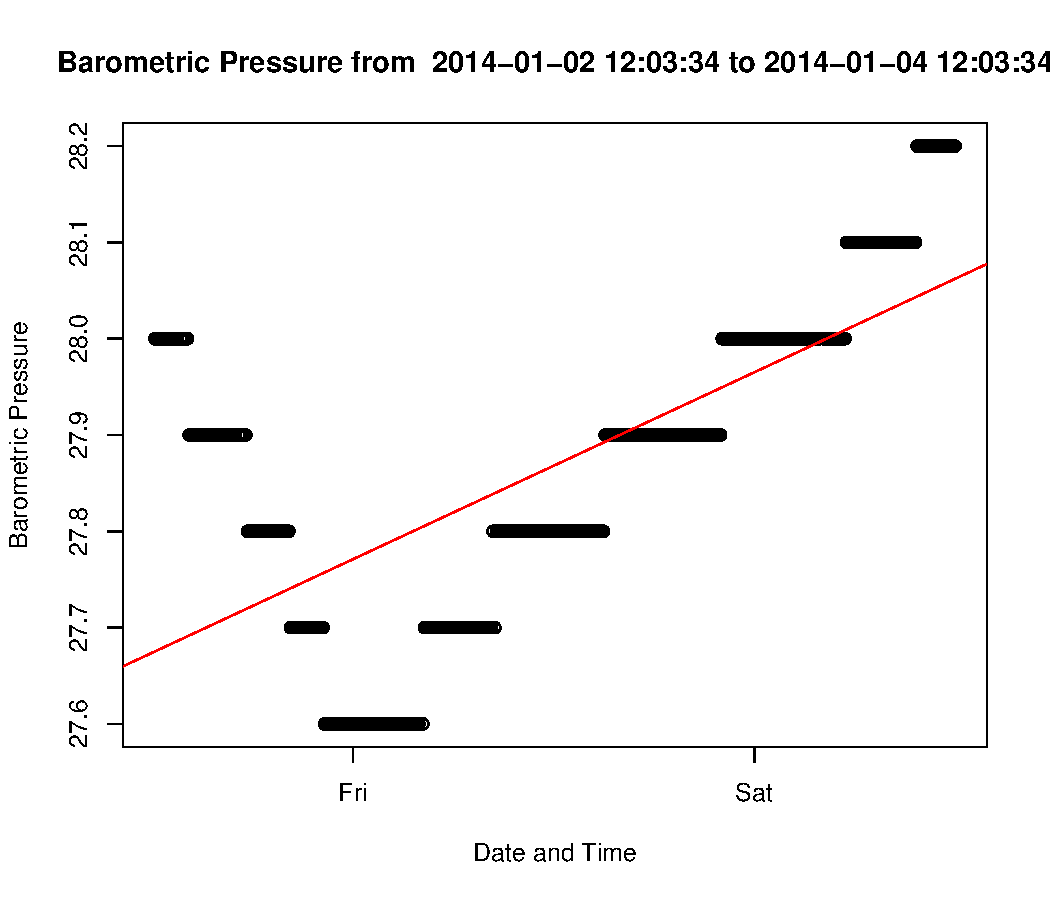
\includegraphics{C:/Users/minhh/Box Sync/R/Master R for Data Science/Code-Clinic-R/output/summarizeTheWeather_files/figure-latex/unnamed-chunk-5-1.pdf}

\end{document}
